\section{Conexión y Compacidad}\label{sec:Rel3}

\begin{ejercicio}
Demuestra que $ \bb{S}^1 $ no es homeomorfo a ningún subconjunto de $ \bb{R} $ ambos considerados con la topología usual.\\


    Sea $A\subset \bb{R}$, y supongamos que $A$ es homeomorfo a $\bb{S}^1$, por lo que existe un homeomorfismo $f:\bb{S}^1 \to A$.
    Como $\bb{S}^1$ sabemos que es conexo, entonces $A$ también lo es, y como $A\subset \bb{R}$, entonces $A$ es un intervalo, supongamos de extremos
    $a$ y $b$, $a<b$, $a,b\in \bb{R}$, o $\pm \infty$.

    Sea ahora $c\in A$ tal que $a<c<b$, y como $f$ es biyectiva, consideremos su preimagen $f^{-1}(c)\in \bb{S}^1$.
    Sea entonces la restricción de $f$ a $\bb{S}^1\setminus \{f^{-1}(c)\}$,
    que es un homeomorfismo entre $\bb{S}^1\setminus \{f^{-1}(c)\}$ y $A\setminus \{c\}$. Como la esfera sin un punto es homeomorfa a $\bb{R}$ (conexo),
    entonces es $A\setminus \{c\}\subset \cc{R}$ es conexo, por lo que es un intervalo. No obstante, esto es una contraddicción,
    ya que $A\setminus \{c\}$ no es un intervalo por tener $a,b\in A\setminus \{c\}$ y $c\notin A\setminus \{c\}$.

\end{ejercicio}

\begin{ejercicio}
Demuestra que $ A=\bb{R}^{n+1} \setminus \bb{S}^n $ no es conexo.\\

    Sea $U=\bb{R}^{n+1}\setminus \ol{B}(0,1)$, $V=B(0,1)$. Tenemos que $U,V\in \T_u$ abiertos de la topología usual de $\bb{R}^{n+1}$.
    Además, $U\cap A=U$ y $V\cap A=V$, por lo que $U,V\in \T_A$ abiertos en la topología usual inducida en $A$. Además, tenemos que $U,V\neq A,\emptyset$.

    Tenemos que $U\cap V=\left(\bb{R}^{n+1}\setminus \ol{B}(0,1)\right) \cap B(0,1)=\emptyset$, y:
    \begin{equation*}
        U\cup V
        = \left(\bb{R}^{n+1}\setminus \ol{B}(0,1)\right) \cup B(0,1)
        = \bb{R}^{n+1} \setminus \bb{S}^n
        = A
    \end{equation*}
    Por tanto, $A$ es conexo.

\end{ejercicio}

\begin{ejercicio}
    Sea $(X, \T)$ un espacio topológico. Demuestra que son equivalentes:
    \begin{enumerate}
        \item $(X, \T)$ es conexo.
        \item Para todo $A \subseteq X$ tal que $\partial A = \emptyset$ se tiene $A = X$ o $A = \emptyset$.
    \end{enumerate}

    Veamos en primer que lugar que, dado $A\subset X$, se tiene que $\partial A=\emptyset$ si y solo si $A$ es abierto y cerrado.
    \begin{description}
        \item[$\Longrightarrow)$]  Supongamos que $\partial A=\emptyset$. Entonces,
        \begin{equation*}
            \emptyset = \partial A = \ol{A} \setminus A^\circ \Longleftrightarrow \ol{A} \subset A^\circ
        \end{equation*}
        Como $A^\circ \subset A\subset \ol{A}$, entonces $A^\circ = \ol{A} = A$, por lo que $A$ es cerrado y abierto.

        \item[$\Longleftarrow)$] Supongamos que $A$ es abierto y cerrado. Entonces,
        \begin{equation*}
            \partial A = \ol{A} \setminus A^\circ = A \setminus A = \emptyset
        \end{equation*}
        Por tanto, $\partial A=\emptyset$.
    \end{description}

    Tenemos por tanto las siguientes equivalencias:
    \begin{enumerate}
        \item $(X, \T)$ es conexo.
        \item Para todo $A \subseteq X$ tal que $A$ es abierto y cerrado se tiene $A = X$ o $A = \emptyset$.
        \item Para todo $A \subseteq X$ tal que $\partial A = \emptyset$ se tiene $A = X$ o $A = \emptyset$.
    \end{enumerate}
    La equivalencia entre 1) y 2) se ha demostrado en la Caracterización de la Conexión, y la equivalencia entre 2) y 3) se ha demostrado en este ejercicio.
\end{ejercicio}

\begin{ejercicio}
    Sean $A$ y $B$ subconjuntos conexos de un espacio topológico $(X, \T)$ tales que $\ol{A} \cap B = \emptyset$. Demuestra que $A \cup B$ es conexo.\\

    Como $\ol{A}\cap B\neq \emptyset$, entonces $\exists b_0\in \ol{A}\cap B$. Como $A$ es conexo y $A\subset A\cup \{b_0\}\subset \ol{A}$, por el Teorema \ref{teo:AdherenciaConexo}
    tenemos que $A\cup \{b_0\}$ es conexo.

    Tenemos que $A\cup B = \left(A\cup \{b_0\}\right)\cup B$, siendo ambos conexos. Además, como se tiene que $b_0\in \left(A\cup \{b_0\}\right)\cap B\neq \emptyset$, por el Teorema \ref{prop:UnionConexos}, $A\cup B$ es conexo.
\end{ejercicio}

\begin{ejercicio}
    Sean $A$ y $B$ subconjuntos cerrados y no vacíos de un espacio $(X, \T)$ tales que $A \cup B$ y $A \cap B$ son conexos. Demuestra que $A$ y $B$ son conexos.\\

    Supongamos que $A$ no es conexo, por lo que existen $C,D\in C_{\T_A}$ cerrados de $A$ no triviales tales que $C\cap D = \emptyset$ y $C\cup D = A$.
    Por ser cerrados de $A$, existen $C',D'\in C_{\T}$ tales que $C=C'\cap A$ y $D=D'\cap A$,
    y como $A\in C_{\T}$ y la intersección de cerrados en cerrado, tenemos que $C,D\in C_\T$.

    Consideramos ahora $A\cap B\subset A=C\cap D$. Veamos ahora que $A\cap B$ solo interseca a uno de los dos conjuntos $C$ y $D$.
    Por contrarecíproco, supongamos $(A\cap B)\cap C\neq \emptyset$ y $(A\cap B)\cap D\neq \emptyset$. Entonces, sean $\wt{C}=(A\cap B)\cap C$ y $\wt{D}=(A\cap B)\cap D$, ambos no vacíos.
    Tenemos que $\wt{C},\wt{D}\in C_{\T_{A\cap B}}$. Además:
    \begin{gather*}
        \wt{C}\cap \wt{D}
        = [(A\cap B)\cap C] \cap [(A\cap B)\cap D] \subset C\cap D = \emptyset \\
        \wt{C}\cup \wt{D}
        = [(A\cap B)\cap C] \cup [(A\cap B)\cap D]
        = (A\cap B)\cap (C\cup D) = (A\cap B)\cap A = A\cap B
    \end{gather*}
    Por tanto, tenemos que $\wt{C},\wt{D}\in C_{\T_{A\cap B}}$ cerrados de $A\cap B$ no triviales tales que $\wt{C}\cap \wt{D}=\emptyset$ y $\wt{C}\cup \wt{D}=A\cap B$,
    por lo que $A\cap B$ no es conexo, lo que es una contradicción.

    Por tanto, $A\cap B\subset C$ o $A\cap B\subset D$.
    Supongamos sin pérdida de generalidad que $A\cap B\subset C$.
    Entonces, $A\cap B\subset C$, y como $C\cap D=\emptyset$, entonces $(A\cap B)\cap D = \emptyset$. Como $D\subset A$, entonces $B\cap D=\emptyset$. Entonces:
    \begin{gather*}
        A\cup B = (C\cup D)\cup B = D \cup (C\cup B)\\
        D\cap (C\cup B) = (D\cap C) \cup (D\cap B) = \emptyset \cup \emptyset = \emptyset
    \end{gather*}
    Como $D$ es no trivial, entonces $C\cup B$ es no trivial. Además, como $C,D,B\subset A\cup B$ y los tres son cerrados, tenemos que $D,C,B\in C_{\T_{A\cup B}}$.
    Como la unión finita de cerrados es cerrado, entonces $C\cup B\in C_{\T_{A\cup B}}$. Por tanto, tenemos una partición de $A\cup B$ en dos cerrados no triviales,
    por lo que $A\cup B$ no es conexo, lo que es una contradicción.
    
    Por tanto, $A$ es conexo. Intercambiando $A$ por $B$, se demuestra que $B$ es conexo.
\end{ejercicio}

\begin{ejercicio} \label{ej:Rel3.6}
    Sean $Y_1$ y $Y_2$ subespacios de $(X, \T)$ y sea $A \subseteq Y_1 \cap Y_2$.
    Demuestra que si $A$ es abierto (respectivamente cerrado) en $Y_1$ y en $Y_2$, entonces $A$ es abierto (respectivamente cerrado) en $Y_1 \cap Y_2$ y en $Y_1 \cup Y_2$.\\

    Como $A\in \T_{Y_1}$, tenemos que $\exists A_1\in \T$ tal que $A=A_1\cap Y_1$. Análogamente, $\exists A_2\in \T$ tal que $A=A_2\cap Y_2$. Notemos que $A_1\cup A_2, A_1\cap A_2\in \T$.

    Como $A_1\cup A_2\in \T$, tenemos que $(A_1\cup A_2)\cap (Y_1\cap Y_2)\in \T_{Y_1\cap Y_2}$. Además,
    \begin{align*}
        (A_1\cup A_2)\cap (Y_1\cap Y_2) &= (A_1\cap Y_1 \cap Y_2)\cup (A_2\cap Y_1\cap Y_2) =\\&= (A\cap Y_2) \cup (A\cap Y_1) = A \cap (Y_1\cup Y_2) = A
    \end{align*}
    Por tanto, $A\in \T_{Y_1\cap Y_2}$. Además, como $A_1\cap A_2\in \T$, tenemos que $(A_1\cap A_2)\cap (Y_1\cup Y_2)\in \T_{Y_1\cup Y_2}$. Además,
    \begin{align*}
        (A_1\cap A_2)\cap (Y_1\cup Y_2) &= (A_1\cap A_2 \cap Y_1)\cup (A_1\cap A_2 \cap Y_2) =\\&= (A\cap A_2) \cup (A\cap A_1) = A \cap (A_1\cup A_2) = A
    \end{align*}
    donde he empleado que $A \subset A_1,A_2$, por lo que $A\subset A_1\cup A_2$. Por tanto, $A\in \T_{Y_1\cup Y_2}$.

    Por tanto, hemos visto que $A\in \T_{Y_1\cap Y_2}$ y $A\in \T_{Y_1\cup Y_2}$, por lo que $A$ es abierto en $Y_1\cap Y_2$ y en $Y_1\cup Y_2$. La demostración para cerrados es análoga,
    ya que la intersección y la unión de dos cerrados es cerrado.
\end{ejercicio}

\begin{ejercicio}
    Sean $(X, \T)$ un espacio conexo y $A$ un subconjunto conexo y no vacío de $X$. Sea $U$ un abierto y cerrado en $X \setminus A$. Demuestra que $A \cup U$ es conexo.

    Supongamos que es disconexo, por lo que existe $V\in \T_{A\cup U}\cap C_{\T_{A\cup U}}$ abierto y cerrado de $A\cup U$ no trivial ($V\neq \emptyset,~V\neq A\cup U$).
    Como $V\in \T_{A\cup U}$, entonces $\exists V'\in \T$ tal que $V=V'\cap (A\cup U)$. Por tanto, $A\cap V = A\cap V'\cap (A\cup U) = A\cap V'$, por lo que $A\cap V\in \T_A$.
    Análogamente, se ve que $A\cap V\in C_{\T_A}$, por lo que $A\cap V$ es abierto y cerrado de $A$ no trivial. Como $A$ es conexo, entonces $A\cap V$ es trivial, por lo que $A\cap V=\emptyset$ o $A\cap V=A$.
    \begin{enumerate}
        \item Supongamos $A\cap V=\emptyset$.
        
        Como $U\subset X\setminus A$ y $V\subset A\cup U$, entonces $V\subset U$. Además, $U\cap V = U\cap V'$, por lo que $V=U\cap V\in \T_{U}$.
        Análogamente, $V\in C_{\T_{U}}$, por lo que $V\in \T_{U}\cap C_{\T_{U}}$. Como $U\in \T_{X\setminus A}\cap C_{\T_{X\setminus A}}$,
        entonces $V\in \T_{X\setminus A}\cap C_{\T_{X\setminus A}}$, por lo que $V$ es abierto y cerrado de $X\setminus A$.

        Aplicamos ahora el Ejercicio \ref{ej:Rel3.6} al conjunto $V$, con $Y_1=X\setminus A$, $Y_2=U\cup A$. Tenemos que $V\subset U\subset Y_1 \cap Y_2$, y
        $V\in \T_{Y_1}\cap C_{\T_{Y_1}}$ y $V\in \T_{Y_2}\cap C_{\T_{Y_2}}$. Por tanto, $V\in \T_{Y_1\cup Y_2}\cap C_{\T_{Y_1\cup Y_2}}$. Calculemos ahora $Y_1\cup Y_2$:
        \begin{equation*}
            Y_1\cup Y_2 = (X\setminus A) \cup (U\cup A) = X
        \end{equation*}
        
        Por tanto $V\in \T\cap C_{\T}$. Como $(X,\T)$ es conexo, entonces $V$ es trivial, por lo que $V=\emptyset$ o $V=X$.
        Como $\emptyset \neq A \subset X$ y $A\cap V=\emptyset$, entonces $V\neq X$, por lo que $V=\emptyset$, lo que es una contradicción.

        \item Supongamos $A\cap V=A$.
        
        Sea $C=(A\cup U)\setminus V\in \T_{A\cup U}\cap C_{\T_{A\cup U}}$. Por tanto, $A\cap C \in \T_A\cap C_{\T_A}$, por lo que $A\cap C$ es abierto y cerrado de $A$, y como $A$ es conexo, entonces $A\cap C$ es trivial.
        Veamos que $A\cap C\neq A$. Tenemos que:
        \begin{equation*}
            A \cap C = A\Longleftrightarrow A\subset C \Longleftrightarrow A\cap V \subset (A\cup U)\setminus V \Longleftrightarrow A\cap V = \emptyset
        \end{equation*}
        Que no es el caso, por lo que $A\cap C\neq A$. Por tanto, $A\cap C=\emptyset$. Aplicando el apartado anterior a $A\cap C$, tenemos que $C=\emptyset$, por lo que $A\cup U \subset V$. No obstante, sabemos que
        $V\subset A\cup U$, por lo que $A\cup U = V$, lo que es una contradicción.
    \end{enumerate}
\end{ejercicio}

\begin{ejercicio}
    Sean $(X, \T)$ un espacio conexo y $A$ un subconjunto conexo y no vacío de $X$. Sea $C$ una componente conexa de $X \setminus A$. Demuestra que $X \setminus C$ es conexo.\\

    Supongamos que $X\setminus C$ es disconexo, por lo que existe $U \in \T_{X\setminus C}\cap C_{\T_{X\setminus C}}$ abierto y cerrado de $X\setminus C$
    no trivial. Como $U\in \T_{X\setminus C}$, entonces $\exists U'\in \T$ tal que $U=U'\cap (X\setminus C)$. Por tanto, $A\cap U=A\cap (X\setminus C) \cap U' = A\cap U'$, donde he aplicado que,
    como $C\subset X\setminus A$, entonces $A\subset X\setminus C$. Por tanto, $A\cap U\in \T_A$. Análogamente, se ve que $A\cap U\in C_{\T_A}$, por lo que $A\cap U$ es abierto y cerrado de $A$. Como $A$ es conexo,
    entonces $A\cap U$ es trivial, por lo que $A\cap U=\emptyset$ o $A\cap U=A$.
    \begin{enumerate}
        \item Supongamos $A\cap U=A$. Entonces, $A\subset U$, y por tanto $A\cap X\setminus (U\cup C) = \emptyset$. Como $C\subset X\setminus A$ y $X\setminus (U\cup C)\subset X\setminus A$, entonces
        $C\subset C\cup X\setminus (U\cup C) \subset X\setminus A$, por lo que $A\cap \left(C\cup X\setminus (U\cup C)\right) = \emptyset$.

        % // TODO: Terminar demostración

        \item Supongamos $A\cap U=\emptyset$. Entonces, $A\subset X\setminus U$, y como $A\subset X\setminus C$, entonces $A\subset X\setminus (U\cup C)$.
    \end{enumerate}
\end{ejercicio}

\begin{ejercicio}
    Prueba que el interior y la frontera de un subconjunto conexo no son en general conexos.\\

    Sea $(\bb{R}^2,\T_u)$ el espacio topológico. Sean $A=\ol{B}[(-1,0), 1], B=\ol{B}[(1,0), 1]\subset \bb{R}^2$ dos bolas cerradas. Estas son convexas, luego son conexos. Además, $A\cap B=\{(0,0)\}\neq \emptyset$, por lo que
    $A\cup B$ es conexo. Sin embargo, $[A\cup B]^\circ=B[(-1,0),1] \cup B[(1,0),1]$, que no es conexo por ser unión de dos abiertos disjuntos.

    Para el caso de la frontera, consideremos $A=[0,1]\times \bb{R}$. Tenemos que es conexo por ser producto de conexos.
    No obstante, $\partial A = (\{0\}\times \bb{R}) \cup (\{1\}\times \bb{R})$, que no es conexo por ser unión de dos cerrados disjuntos.


\end{ejercicio}

\begin{ejercicio}
    Sean $(X, \T)$ y $(X', \mathcal{T'})$ dos espacios topológicos conexos y $A \subseteq X$, $A\neq X$, $B \subseteq X'$, $B\neq X'$. ¿Es $(X \times X') \setminus (A \times B)$ conexo?

    % // TODO: Terminar demostración (no sé si es cierta)
\end{ejercicio}

\begin{ejercicio}
    Sea $X$ el conjunto de los puntos de $ \bb{R}^2 $ con alguna coordenada racional. Prueba que $X$ con la topología inducida es un subconjunto conexo.\\

    Sea $X=\{(x,y)\in \bb{R}^2 \mid x\in \bb{Q} \lor y\in \bb{Q}\}=(\bb{R}\times \bb{Q}) \cup (\bb{Q}\times \bb{R})$.
\end{ejercicio}

\begin{ejercicio}
    Prueba que no existen aplicaciones continuas e inyectivas de $\bb{R}^2$ en $\bb{R}$.

    Sea $f:\bb{R}^2\to \bb{R}$ continua e inyectiva. Tenemos que, como $f$ es continua y $\bb{R}^2$ es conexo, $f(\bb{R}^2)\subset \bb{R}$ es conexo, luego es un intervalo, supongamos de extremos
    $a$ y $b$, $a<b$, $a,b\in \bb{R}$, o $\pm \infty$.

    Sea ahora $c\in f(\bb{R}^2)$ tal que $a<c<b$, y como $f$ es inyectiva, consideremos su preimagen $f^{-1}(c)\in \bb{R}^2$, que es única.
    Sea entonces la restricción de $f$ a $\bb{R}^2\setminus \{f^{-1}(c)\}$,
    que es un homeomorfismo entre $\bb{R}^2\setminus \{f^{-1}(c)\}$ y $A\setminus \{c\}$. Como $\bb{R}^2\setminus \{f^{-1}(c)\}$ es homeomorfo a $\bb{R}^2\setminus \{0\}$, es conexo, por lo que
    $A\setminus \{c\}\subset \bb{R}$ es conexo pero no es un intervalo, ya que $a,b\in A\setminus \{c\}$ y $c\notin A\setminus \{c\}$, lo que es una contradicción.
\end{ejercicio}

\begin{ejercicio}
    Sea $(X, \T)$ un espacio topológico y $\{A_i\}_{i \in I}$ una partición por subconjuntos conexos y abiertos de $(X, \T)$. Entonces $\{A_i\}_{i \in I}$ es la familia de componentes conexas de $X$.\\

    Demostrado en la Proposición \ref{prop:ParticionConexosAbiertos}.
\end{ejercicio}



\begin{ejercicio}
    Sea $ X = \{a, b, c, d, e\} $ y $ \T = \{X, \emptyset, \{a\}, \{c, d\}, \{a, c, d\}, \{b, c, d, e\}\} $. Calcula las componentes conexas de $(X, \T)$.

    \begin{equation*}
        \left\{\{a\}, \{b, c, d, e\}\right\}
    \end{equation*}
    Dicho conjunto tenemos que es una partición de $X$ por subconjuntos conexos y abiertos, por lo que son las componentes conexas de $(X, \T)$.
\end{ejercicio}

\begin{ejercicio}
    Denotemos por $ C((a, b), r) $ la circunferencia en $ \bb{R}^2 $ con centro $(a, b)$ y radio $r$. Demuestra que ninguno de los siguientes espacios topológicos es homeomorfo a cualquier otro:
    \begin{enumerate}
        \item $ X_1 = C((0, 0), 1) $
        \item $ X_2 = C((-1, 0), 1) \cup C((1, 0), 1) $
        \item $ X_3 = C((-1, 0), 1) \cup C((1, 0), 1) \cup C\left(\left(0, \sqrt{3}\right), 1\right) $
        \item $ X_4 = C((-1, 0), 1) \cup C((1, 0), 1) \cup (\bb{R} \times \{1\}) $.
    \end{enumerate}
    \begin{figure}[H]
        \begin{subfigure}[c]{0.5\linewidth}
            \centering
            \begin{tikzpicture}
                % Ejes cartesianos
                \draw[-stealth, dashed] (-1.5, 0) -- (1.5, 0) node[right] {$x$};
                \draw[-stealth, dashed] (0, -1.5) -- (0, 1.5) node[above] {$y$};

                % Circunferencia
                \draw[teal] (0, 0) circle (1);
            \end{tikzpicture}
            \caption{$X_1 = C((0, 0), 1)$}
        \end{subfigure}\hfill
        \begin{subfigure}[c]{0.5\linewidth}
            \centering
            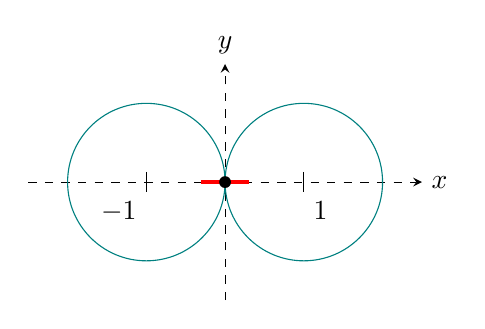
\begin{tikzpicture}
                % Ejes cartesianos
                \draw[-stealth, dashed] (-2.5, 0) -- (2.5, 0) node[right] {$x$};
                \draw[-stealth, dashed] (0, -1.5) -- (0, 1.5) node[above] {$y$};

                % Circunferencia
                \draw[teal] (-1, 0) circle (1);
                \draw[teal] (1, 0) circle (1);

                % Marca de punto de tangencia
                \draw[ultra thick, red] (-0.3,0) -- (0.3,0);
                \fill (0,0) circle (0.075);

                % Etiqueta en x=1, x=-1
                \draw (1,0.13) -- (1,-0.13) node[below right] {$1$};
                \draw (-1,0.13) -- (-1,-0.13) node[below left] {$-1$};
            \end{tikzpicture}
            \caption{$X_2 = C((-1, 0), 1) \cup C((1, 0), 1)$}
        \end{subfigure}\hfill
        \begin{subfigure}[c]{0.5\linewidth}
            \centering
            \begin{tikzpicture}
                % Ejes cartesianos
                \draw[-stealth, dashed] (-2.5, 0) -- (2.5, 0) node[right] {$x$};
                \draw[-stealth, dashed] (0, -1.7) -- (0, 3.3) node[above] {$y$};

                % Cálculo de raiz de 3
                \pgfmathsetmacro{\raiz}{sqrt(3)}
                
                % Centros de las circunferencias
                \coordinate (C1) at (-1, 0);
                \coordinate (C2) at (1, 0);
                \coordinate (C3) at (0, \raiz);
                % Circunferencia
                \draw[teal] (C1) circle (1);
                \draw[teal] (C2) circle (1);
                \draw[teal] (C3) circle (1);

                % Puntos de tangencia
                \coordinate (P1) at (-0.5, \raiz/2);
                \coordinate (P2) at (0.5, \raiz/2);
                \coordinate (P3) at (0, 0);

                % Marca de punto de tangencia
                \draw[ultra thick, red] ($(C1)!0.7!(P1)$) -- ($(C1)!1.3!(P1)$);
                \draw[ultra thick, red] ($(C2)!0.7!(P2)$) -- ($(C2)!1.3!(P2)$);
                \draw[ultra thick, red] ($(C1)!0.7!(P3)$) -- ($(C1)!1.3!(P3)$);
                \fill (P1) circle (0.075);
                \fill (P2) circle (0.075);
                \fill (P3) circle (0.075);

                % Etiqueta en x=1, x=-1
                \draw (1,0.13) -- (1,-0.13) node[below right] {$1$};
                \draw (-1,0.13) -- (-1,-0.13) node[below left] {$-1$};

                % Etiqueta en y=sqrt(3)
                \draw (0.13, \raiz) -- (-0.13, \raiz) node[left] {$\sqrt{3}$};
            \end{tikzpicture}
            \caption{\centering $X_3~=~C((-1, 0), 1) \cup C((1, 0), 1) \cup C\left(\left(0, \sqrt{3}\right), 1\right)$}
        \end{subfigure}
        \begin{subfigure}[c]{0.5\linewidth}
            \centering
            \begin{tikzpicture}
                % Ejes cartesianos
                \draw[-stealth, dashed] (-2.5, 0) -- (2.5, 0) node[right] {$x$};
                \draw[-stealth, dashed] (0, -1.5) -- (0, 1.5) node[above] {$y$};
                
                % Centros de las circunferencias
                \coordinate (C1) at (-1, 0);
                \coordinate (C2) at (1, 0);
                % Circunferencia
                \draw[teal] (C1) circle (1);
                \draw[teal] (C2) circle (1);

                \draw[teal] (-2.5, 1) -- (2.5, 1) node[right] {$y=1$};

                % Puntos de tangencia
                \coordinate (P1) at (-1,1);
                \coordinate (P2) at (1,1);

                % Marca de punto de tangencia
                \draw[ultra thick, red] ($(C1)!0.7!(P1)$) -- ($(C1)!1.3!(P1)$);
                \draw[ultra thick, red] ($(C2)!0.7!(P2)$) -- ($(C2)!1.3!(P2)$);
                \fill (P1) circle (0.075);
                \fill (P2) circle (0.075);

                % Etiqueta en x=1, x=-1
                \draw (1,0.13) -- (1,-0.13) node[below right] {$1$};
                \draw (-1,0.13) -- (-1,-0.13) node[below left] {$-1$};
            \end{tikzpicture}
            \caption{\centering $X_4~=~C((-1, 0), 1) \cup C((1, 0), 1) \cup (\bb{R} \times \{1\}) $}
        \end{subfigure}
    \end{figure}

    Veamos en primer que, toda circunferencia a la que se le quita un punto sigue siendo conexa. 

    Veamos en primer lugar que $X_1$ no es homeomorfo al resto. Supongamos que $f_i:X_1\to X_i$ es un homeomorfismo para $i=2,3,4$.
    Sean $p_i,q_i\in X_i$ tales que $p_i\neq q_i$ para $i=2,3,4$, no perteneciendo ambos a la misma circunferencia ni, en el caso de $X_4$, a la recta $y=1$.
    Entonces, $f_i^{-1}(p_i),f_i^{-1}(q_i)\in X_1$ son tales que $f_i^{-1}(p_i)\neq f_i^{-1}(q_i)$ por ser $f_i$ inyectiva.

    La restricción de $f_i$ a $X_1\setminus \{f_i^{-1}(p_i), f_i^{-1}(q_i)\}$ es un homeomorfismo entre
    $X_1\setminus \{f_i^{-1}(p_i), f_i^{-1}(q_i)\}$ y $X_i\setminus \{p_i,q_i\}$. Como $p_i,q_i$ no son puntos de tangencia, entonces
    $X_i\setminus \{p_i,q_i\}$ es conexo, ya que para todo $i$ 
\end{ejercicio}

\begin{ejercicio}
Decide cuáles de los siguientes subespacios de $ \bb{R} $ y $ \bb{R}^2 $ son compactos. Razona la respuesta:
\begin{enumerate}
    \item $ [0, \infty[ $
    \item $ [0, 1] \cap \mathbb{Q} $
    \item $ \{(x, y) \in \bb{R}^2 \mid x \geq 1, 0 \leq y \leq \frac{1}{x}\} $
    \item $ \{(x, y) \in \bb{R}^2 \mid |x| + |y| \leq 1\} $
    \item $ \bb{S}^1 \setminus \left\{\left(\frac{\sqrt{2}}{2}, -\frac{\sqrt{2}}{2}\right)\right\} $
    \item $ (]0, 1[, \T) $ donde $ \T = \{\emptyset, X\} \cup \{]0, 1 - \frac{1}{n}[~\mid n \geq 2\} $
    \item $ (\bb{R}, \T) $ donde $ \T = \{O \subseteq \bb{R} \mid O = U \setminus B, U \in \T_u, B \subseteq \left\{\frac{1}{n} \mid n \in \mathbb{N}\right\}\} $
    \item La recta de Sorgenfrey.
    \item $ (\mathbb{Q}, {\T_u}_{\big |\mathbb{Q}}) $
    \item $ X $ es un conjunto, $ p \in X $ un punto fijo y $ \T = \{O \subseteq X \mid p \in O\} \cup \{\emptyset\} $.
    \item $ X $ es un conjunto, $ p \in X $ un punto fijo y $ \T = \{O \subseteq X \mid p \in O\} \cup \{X\} $.
    \item $ \mathbb{N} $ con la topología $ \T = \{\emptyset, \mathbb{N}\} \cup \{\{1, \ldots, n\} \mid n \in \mathbb{N}\} $.
\end{enumerate}
\end{ejercicio}

\begin{ejercicio}
Sea $(X, \T)$ un espacio topológico. Prueba que si $ A, A' \subseteq X $ son subespacios compactos, entonces $ A \cup A' $ también es compacto.
\end{ejercicio}


\begin{ejercicio}
Sea $(X, \T)$ un espacio topológico Hausdorff. Prueba que si $\{A_i\}_{i \in I}$ son subespacios compactos de $X$, entonces $\bigcap\limits_{i \in I} A_i$ también es compacto.
\end{ejercicio}

\begin{ejercicio}
Sea $(X, \T)$ un espacio topológico compacto y supongamos que para cada $n \in \mathbb{N}$, $C_n$ es un subconjunto cerrado y no vacío tal que $C_{n+1} \subseteq C_n$. Prueba que $\bigcap\limits_{n=1}^{\infty} C_n \neq \emptyset$.
\end{ejercicio}

\begin{ejercicio}
Sea $(X, \T)$ un espacio Hausdorff y compacto y $f: X \to X$ una aplicación continua. Prueba que existe $A \subseteq X$ un subconjunto cerrado y no vacío tal que $f(A) = A$.
\end{ejercicio}

\begin{ejercicio}
Demuestra el siguiente resultado conocido como el \emph{teorema de la aplicación contractiva}: si $X$ es un espacio métrico compacto y $f: X \to X$ es una aplicación contractiva (es decir, existe $K < 1$ tal que $d(f(x), f(y)) \leq K \cdot d(x, y)$ para todo $x, y \in X$), entonces existe un único punto $x \in X$ tal que $f(x) = x$.
\end{ejercicio}

\begin{ejercicio}
Sea $(X, \T)$ un espacio topológico Hausdorff y $\{K_n\}_{n \in \mathbb{N}}$ una sucesión estrictamente decreciente de compactos no vacíos en $X$. Demuestra que $K = \bigcap\limits_{n \in \mathbb{N}} K_n \neq \emptyset$ y que si $U \in \T$ tal que $K \subseteq U$, entonces existe $m \in \mathbb{N}$ tal que $K_m \subseteq U$.
\end{ejercicio}

\begin{ejercicio}
Encuentra contraejemplos de las afirmaciones siguientes:
\begin{enumerate}
\item En cualquier espacio métrico toda bola cerrada es un subespacio compacto.
\item En cualquier espacio métrico ninguna bola abierta puede ser un subespacio compacto.
\end{enumerate}
\end{ejercicio}

\begin{ejercicio}
Demuestra que no existe ninguna función continua \[f: ([0, 1], \T_u|[0,1]) \to (\bb{R}, \T_u)\] que verifique $f(x) \in \bb{R} \setminus \mathbb{Q}$ si $x \in \mathbb{Q}$ y $f(x) \in \mathbb{Q}$ si $x \in \bb{R} \setminus \mathbb{Q}$.
\end{ejercicio}

\begin{ejercicio}
Sean $(X, \T)$ e $(Y, \mathcal{T'})$ espacios topológicos con $(X, \T)$ compacto. Prueba que la proyección $\pi_Y: X \times Y \to Y$ es cerrada.
\end{ejercicio}

\begin{ejercicio}
Se dice que $C \subseteq \bb{R}^2$ es una curva de Jordan si $C = f([0, 1])$ para $f: [0, 1] \to \bb{R}^2$ una aplicación continua e inyectiva. Prueba que no existe una curva de Jordan que rellene el cuadrado $[0, 1] \times [0, 1]$.
\end{ejercicio}


\begin{ejercicio}
    Prueba que los subconjuntos compactos de la recta de Sorgenfrey son necesariamente
numerables.
\end{ejercicio}